\documentclass{beamer}
\usepackage{tikz}
\usepackage{algorithm}
\usepackage[algo2e]{algorithm2e}
\usepackage[noend]{algpseudocode}
\usecolortheme{orchid}

\mode<beamer>{\setbeamertemplate{blocks}[rounded][shadow=true]}

%\setbeamercolor{block example}{fg=blue, bg=black!20}



\title{Finding Influential People from Historical News Repository}
\author{Aayushee Gupta}
\institute{Indraprastha Institute of Information Technology}
\date{June 19, 2014}
\begin{document}
\maketitle


\AtBeginSection[]
{
\begin{frame}{Agenda}
\tableofcontents[currentsection]
\end{frame}
}
%hideothersubsections
%MOTIVATION
\section{Motivation}
\begin{frame}
\frametitle{Motivation}
 
\begin{itemize}
\item People Search - an important practical application of historical newspapers to find information about people and track the timeline of news articles related to them
\begin{figure}[ht]
\begin{center}
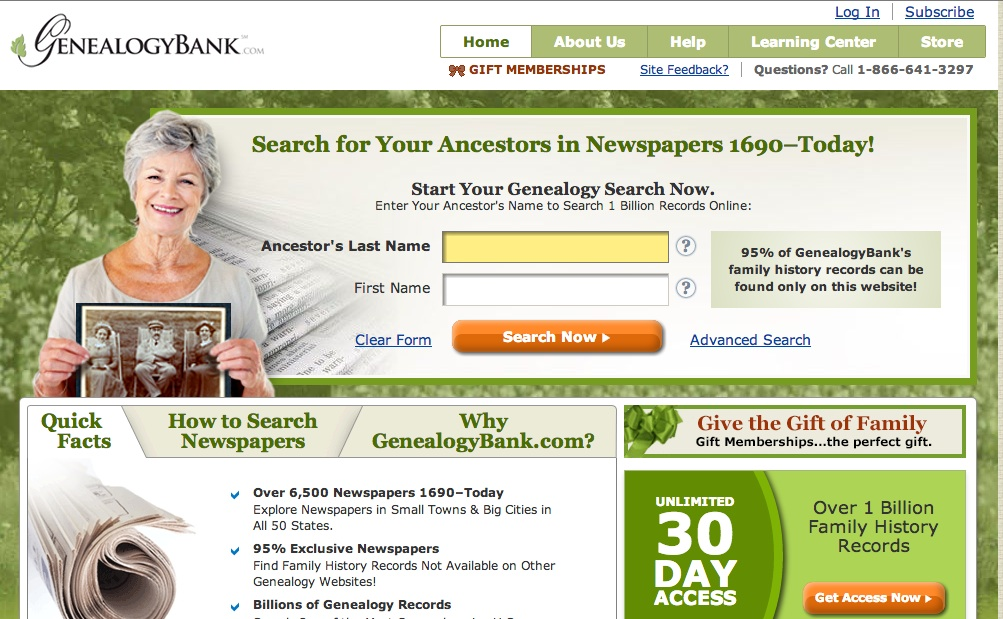
\includegraphics[scale=0.2]{genealogy.jpg}
\end{center}
\end{figure}
\item Finding influential people from historic newspaper archives- a novel problem
\end{itemize}
\end{frame}


%PROBLEM DESCRIPTION
\section{Problem Description}
\begin{frame}
\frametitle{Problem Description}
\textbf{Aim}: To find ``influential" people from historical news OCR archives where
an influential person can be defined as:\\


``A person whose actions and opinions strongly influence a course of events"\\  \vspace{0.5in}

\pause
Divided into subproblems:
\begin{itemize}
\pause
\item Spell Correction and Cleaning of OCR text
\pause
\item Development of a People Gazetteer-an organized structure to ease the process of identification of influential people
\pause
\item Influential People Identification-define the criteria to identify and rank people as ``influential".
\end{itemize}

\end{frame}


%NOVEL CONTRIBUTION
\section{Novel Contribution}
\begin{frame}
\frametitle{Novel Contribution}
\begin{itemize}
\item A novel Spell Correction Evaluation (SCE) algorithm for measuring performance of Spelling Correction
\item Development of People Gazetteer - an organized dictionary of people names and a list of news articles of their occurrence along with the corresponding topic label of each article which can be used to identify and rank influential people
\item Define an Influential Person Index (IPI) and metrics for its calculation to identify and rank influential people from the People Gazetteer
\end{itemize}
\end{frame}


%RELATED WORK
\section{Related Work}
\begin{frame}
\frametitle{Related Work}
\begin{itemize}
\item
GATE gazetteers define gazetteers as set of lists containing names of entities such as cities, organizations, days of week, etc
\item
Gazetteers have been used as a processing resource to find occurrence of entity names in text (Example: Named Entity Recognition)
\item
Influential people identification has been done mostly in the field of social networking, marketing and diffusion research
\item
 Number of votes, tweets, comments, followers, etc are common parameters used for defining influence but no applicable to the newspaper environment 
\end{itemize} 

\end{frame}

 
%SOLUTION FRAMEWORK
\section{Solution Framework}
\begin{frame}

\frametitle{Solution Framework}
\begin{figure}[ht]
\begin{center}
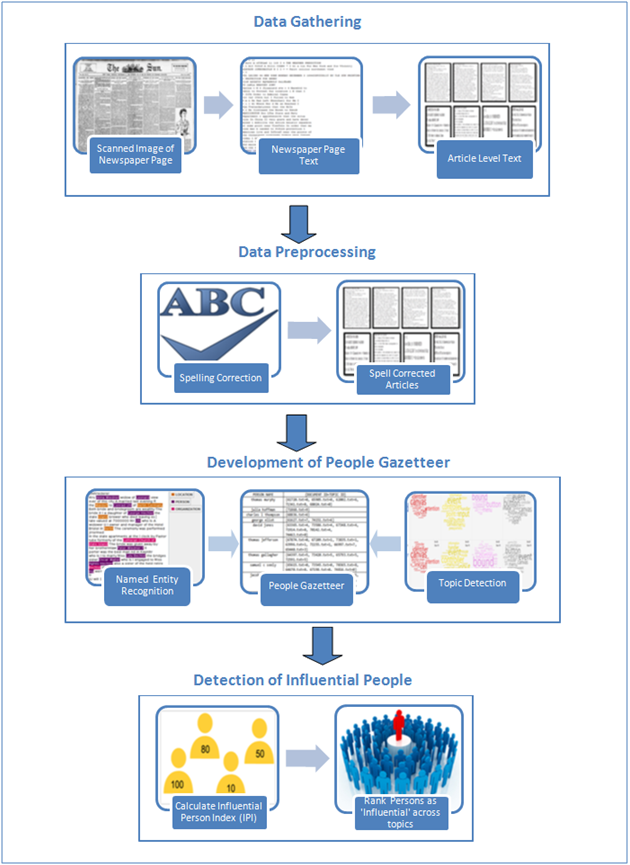
\includegraphics[scale=0.35]{images/framework3.png}
\end{center}
\end{figure}

\end{frame}

%DATA DESCRIPTION
\subsection{Data Gathering}
\tableofcontents[currentsection,currentsubsection]

\begin{frame}

\frametitle{Data Gathering}
\begin{itemize}
\item \textbf{Data Source} : Chronicling America - provides scanned OCR newspaper pages of American newspapers published between 1836 and 1922 
\item \textbf{Data Statistics} : 14020 news articles of ``The Sun" newspaper published between November-December 1894 consisting of 8 million tokens
\item \textbf{Data Characteristics} : News articles consist of one or more OCR errors of the types- Real word, Non-real word, Non-word, Word Split and Join and New line errors
\end{itemize}
\end{frame} 

%DATA PREPROCESSING
\subsection{Data Preprocessing}
\tableofcontents[currentsection,currentsubsection]

\begin{frame}
\frametitle{Data Preprocessing}
\begin{itemize}
\item
Required to deal with OCR errors in the news articles
\item
Edit distance algorithm used for spelling correction of non-real and non-word OCR errors\\ \vspace{0.2in}
Based on levenshtein distance and can correct errors due to substitution, insertion and deletion of at most 2 letters in a word 
\end{itemize}
\end{frame}

\begin{frame}
\frametitle{Spelling Correction Algorithm}
\begin{itemize}
\item ``Edit distance" corresponds to the minimum number of insertion, deletion and substitution required to transform one string into another
\item Precompiled dictionary is used to search for candidate list of words within edit distance 2 from the word to be corrected
 \item Word correction is done by replacement with the highest frequency word and lowest edit distance among the candidate list of words
\item Person name correction is improved by enhancing dictionary with people names by running Stanford NER-CRF parser on subsets of the ClueWeb12 dataset available as a part of TREC 2013 Crowdsourcing track

\end{itemize}
\end{frame}

\begin{frame}[allowframebreaks]
\frametitle{Spelling Correction Evaluation}

\begin{itemize}
\item
Required to measure the performance of spelling correction\\ \vspace{0.2in}
\item
Evaluation Parameters:
\end{itemize}
\begin{enumerate}
\item \alert{ Accuracy} : measures the percentage of actual errors that get corrected in the OCR text after spelling correction and defined as follows:
$$Accuracy=  \dfrac{TP+FP} {TP+ FP + TN + FN}$$


where, 

$TP$=Number of True Positives,

$TN$=Number of True Negatives,

 $FP$=Number of False Positives,

 $FN$=Number of False Negatives.



\item \alert{Time taken} to run Spelling Correction Algorithm
\item \alert{Person Names Detection Rate} (PNDR) : defined as the ratio of person names recognized through Named Entity Recognition (NER) before spelling correction process and the total number of person names recognized in the original newspaper articles
$$PNDR=\dfrac{ \text{Person Names recognized before/after spelling correction}} {\text{ Person Names recognized in original newspaper articles}} $$
\end{enumerate}
\end{frame}


\begin{frame}
\frametitle{Spelling Correction Evaluation (SCE) Algorithm}
\begin{itemize}
\item Word by word correspondence between corrected and original dataset not possible because of Word Split and Join errors in OCR dataset
\item SCE algorithm performs automatic evaluation of word by word post  spelling correction on OCR dataset 
\item Algorithm uses an n-gram words approach by considering a window of k words before and after each word in the original text for each word in the corrected text
\item Each word in the corrected text is marked as a True Positive, True Negative, False Positive, False Negative based on whether the spelling had been corrected and if a match is found in the k words window of the original text
\end{itemize}
\end{frame}


\begin{frame}
    \scalebox{0.65}{\begin{minipage}{1.53846\textwidth}

\begin{algorithm}[H]
\caption{MatchWordGrams function of SCE Algorithm for measuring accuracy }
\begin{algorithmic}
\Function {MatchWordGrams}{OcrLine, CorrectedLine, OriginalLine, jstart, jend, i}
  
 \For{(int j=jstart; j$<$jend; j++)}
  {
    \If{ ((CorrectedLine[i].equals(OriginalLine[j]))\&\&(!(OcrLine[i].equals(CorrectedLine[i]))))}
     {
	  $tp=tp+1$\;
	  flag0=false\;
	 \Return $tp$\;
	  }
	\ElseIf{((CorrectedLine[i].equals(OriginalLine[j]))\&\&(OcrLine[i].equals(CorrectedLine[i])))}
	      {
		 $tn=tn+1$\;
		  flag1=false\;
		\Return $tn$\;
	      }
}

	 \If{(!(OcrLine[i].equals(CorrectedLine[i]))\&\&flag0==true)}
	 {
		    $fp=fp+1$\;
		   \Return $fp$\;
            }
	 
	 \ElseIf{((OcrLine[i].equals(CorrectedLine[i])) \&\& flag1==true)}
	 {
		    $fn=fn+1$\;
		   \Return $fn$\;
	 }
\EndFunction
\end{algorithmic}
\end{algorithm}%
\end{minipage}}
\end{frame}


\begin{frame}
\frametitle{Example}
\begin{block}{Line text from 3 versions of a news article:}
OcrLine= \textit{Irnniluttry iiownllllnu at tilchmond}\\

CorrectedLine= \textit{Irnniluttry iiownllllnu at Richmond}\\

OriginalLine= \textit{Grand jury now sitting at Richmond} 
\end{block}

\begin{table}[bt]
\begin{tabular}{|p{2.5cm}|p{4.5cm}|p{2cm}|} \hline
\textbf{Word in Corrected Line} & \textbf{Corresponding Word Window in Original Line}& \textbf{Result} \\ \hline
Irnniluttry & Grand jury now & FN \\ \hline
iiownllllnu & Grand jury now sitting & FN \\ \hline
at & Grand jury now sitting at & TN \\ \hline
Richmond  &  sitting at Richmond & TP \\ \hline
\end{tabular}
\end{table}
\end{frame}


\subsection{Development of People Gazetteer}
\tableofcontents[currentsection,currentsubsection]
\begin{frame}
\frametitle{Development of People Gazetteer}
Two step process:
\begin{itemize}
\item
Person Named Entity Recognition (PNER)-
 Extraction of person names from the news articles dataset using Named Entity Recognition
\item
Topic Detection-Assignment of topics to news articles using LDA model
\end{itemize}
\end{frame}



\begin{frame}
\frametitle{PNER}
\begin{itemize}
\item
 Stanford CRF-NER used for the process of Named Entity Recognition 
\item
Only multi-term person entities are analyzed
Example: \alert {Henry} is ignored while \alert{Henry Smith} is stored
\item
Inverted Index is created to link person entities with the list of news articles in which they occur
\item
38426 person entities recognized from 14020 news articles 

\end{itemize}
\end{frame}


\begin{frame}
\frametitle{Person Categories}
 Extracted person entities are divided into following categories for separate analysis of each category:
\begin{table}[bt]
\begin{tabular}{|p{3.5cm}|p{3cm}|p{2cm}|} \hline
\textbf{Person Category} & \textbf{Number of news articles}& \textbf{Statistics from dataset} \\ \hline
Marginally Influential & less than 4 & 38066 \\ \hline
Medium Influential & 4 to 15 & 344 \\ \hline
Highly Influential & more than 15 & 16 \\ \hline
\end{tabular}
\end{table}
\end{frame}


\begin{frame}
\frametitle{Topic Detection}
\begin{itemize}
\item
\alert{Topic} : a set of words which describe what any document is about
\item
\alert{Topic Detection}: use topic modelling algorithm for examining a set of documents and discover main topics occurring across the documents as well as the balance of topics in each document based on the statistics of the words in the complete document set
\item
\alert{LDA} :  generative probabilistic model in which documents exhibit multiple topics and each topic is a distribution over a fixed vocabulary
\item
\alert{AD-LDA} : approximate distributed LDA model that uses distributed computation on multiple processors to infer document topics and is faster than the simple LDA approach
\end{itemize}
\end{frame}

\begin{frame}
\frametitle{Topic Model Evaluation}
\end{frame}

\begin{frame}
\frametitle{People Gazetteer Sample Output}
\begin{figure}[ht]
\begin{center}
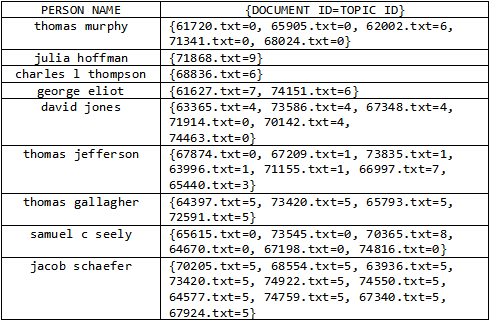
\includegraphics[scale=0.7]{images/gazetteer.png}
\end{center}
\end{figure}
\end{frame}

\subsection{Identifying Influential People}
\tableofcontents[currentsection,currentsubsection]
\begin{frame}
\frametitle{Identification of Influential People}
\begin{itemize}
\item
Define Document Index (DI) to measure effect of each document on a person's influence score
\item
Calculate Influential Person Index (IPI) for each person entity based on the maximum DI in their document list
\item
Rank person entities in decreasing order of IPI
\end{itemize}
\end{frame}

\begin{frame}[allowframebreaks]
\frametitle{Document Index}
\begin{itemize}
\item
Measures how each document in the person entity's associated list of documents affects his influence score
\item
Parameters for estimating DI:
\begin{enumerate}
\item
\alert{ Normalized Document Length} (NDL) : normalized number of tokens contained in a news article

$$\text{ NDL}=\dfrac{\text{Document Length}} {\text{Maximum Document Length in the dataset}}$$

\item
\alert{Normalized Term Frequency} (NTF) : normalized number of occurrences of a person's name in a news article

$\text{NTF}=	1	+\log	$(TF of person entity in current article)

\item  
\alert{Number of similar articles} (NSIM) :  proportion of topic similar articles for a news article in a person's list

$$NSIM= \dfrac{\text{Number of topic similar articles}} {\text{Total number of articles in the person's document list}}$$

\end{enumerate}

\item
Formula for estimating DI:
$$DI = w_a . NDL + w_b . NSIM + w_c . NTF $$

where, $w_a$,$ w_b$ and $w_c$ are the weights associated with each of the parameters NDL, NSIM and NTF respectively

\item
DI is a heuristic measure of these three parameters where each of the parameters can be weighted as per dataset characteristics and user requirements
\end{itemize}
\end{frame}

\begin{frame}
\frametitle{Calculation of IPI}
\begin{itemize}
\item
An index calculated for each person entity in order to measure its influence in the news dataset and calculate its influential score
\item
Formula for calculation:
$$IPI= max DI(d_1, d_2, ...,d_n)+ UniqT$$

where, \\
 $max DI(d_1, d_2, ...,d_n)$ = Maximum Document Index of a document $d_i$ in a person entity's list of  $n$ articles

$$UniqT = \dfrac{\text{Number of Unique Article Topics in a person entity's list}}{\text{Total Number of Topics in the corpus}}$$

\end{itemize}
\end{frame}

\section{Results}
\begin{frame}

\end{frame}

\section{Discussion}
\begin{frame}
\frametitle{Discussion and Future Work}
\begin{itemize}
\item
Spelling Correction algorithm needs to be improved in order to correct other OCR errors like New Line and Word Split and Join errors
\item
Person Named Entity Disambiguation : a hard problem to solve since persons with similar names can occur in multiple topic related articles in newspapers
\item
Co-reference Resolution of person names needs to be performed to link multiple ways in which a single person is addressed to avoid analyzing unnecessary person names
\item
Heuristic-based parameter estimation of IPI can be replaced by an optimization approach such as multiple instance clustering to avoid choosing of parameter weights  and biasing of results 
\end{itemize}
\end{frame}

\section*{References}
\begin{frame}

\end{frame}
\end{document}